\documentclass[a4j]{ujarticle}
\renewcommand{\baselinestretch}{0.85}
\usepackage[top=1.5cm, bottom=1.5cm, left=1.5cm, right=1.5cm]{geometry}
\usepackage{xcolor}
\usepackage[dvipdfmx]{graphicx, hyperref}
\usepackage{listings}
\usepackage{multirow}
\usepackage{siunitx}
\usepackage{subfig}
\usepackage{url}
\usepackage{listings}
\usepackage{caption,stackengine}

\colorlet{punct}{red!60!black}
\definecolor{background}{HTML}{EEEEEE}
\definecolor{delim}{RGB}{20,105,176}
\colorlet{numb}{magenta!60!black}

\newcommand{\Sref}[1]{\mbox{\ref{sec:#1}}}
\newcommand{\Tref}[1]{\mbox{表\ref{tab:#1}}}
\newcommand{\Eref}[1]{\mbox{式(\ref{eq:#1})}}
\newcommand{\Fref}[1]{\mbox{図\ref{fig:#1}}}
\renewcommand{\lstlistingname}{ソースコード}
\newcommand{\Lref}[1]{\mbox{ソースコード\ref{lst:#1}}}
\newcommand{\bhline}[1]{\noalign{\hrule height #1}}

\hypersetup{
	setpagesize=false,
	bookmarksnumbered=true,
	bookmarksopen=true,
	colorlinks=true,
	linkcolor=black,
	citecolor=black
}

\begin{document}
    \begin{flushright}
        MDLab GM資料\\
        22年5月17日(火)
    \end{flushright}

    \begin{center}
        {\Large	腹部超音波画像からの腫瘍検出}
    \end{center}

    \begin{flushright}
        {\large B4 原 英吾}\\
    \end{flushright}

    \section{研究背景および目的}
    \begin{figure}[h]
        \begin{minipage}{.59\textwidth}
            \begin{itemize}
                \item 背景
                \begin{itemize}
                    \item 器具の操作と診断を同時に行わなければならず高難易度
                    \item 肝臓は沈黙の臓器と呼ばれ初期には自覚症状がほとんどない
                    \begin{itemize}
                        \item 症状を自覚している時には重症化している場合が多い
                    \end{itemize}
                    \item 機械学習による診断のサポート
                    \begin{itemize}
                        \item 良性・悪性を見分けることが重要視される
                        \item \Fref{ex}の様に明らかなラベル不足\footnotemark[1]のある画像が存在する
                    \end{itemize}
                \end{itemize}
                \item 目的
                \begin{itemize}
                    \item 既存の研究を踏まえたモデルの精度向上
                    \begin{itemize}
                        \item 良性・悪性判別の高精度化
                    \end{itemize}
                    \item 超音波支援システムの開発
                    \begin{itemize}
                        \item 早期発見につながると良い
                    \end{itemize}
                \end{itemize}
            \end{itemize}
        \end{minipage}
        \begin{minipage}{.39\textwidth}
            \centering
            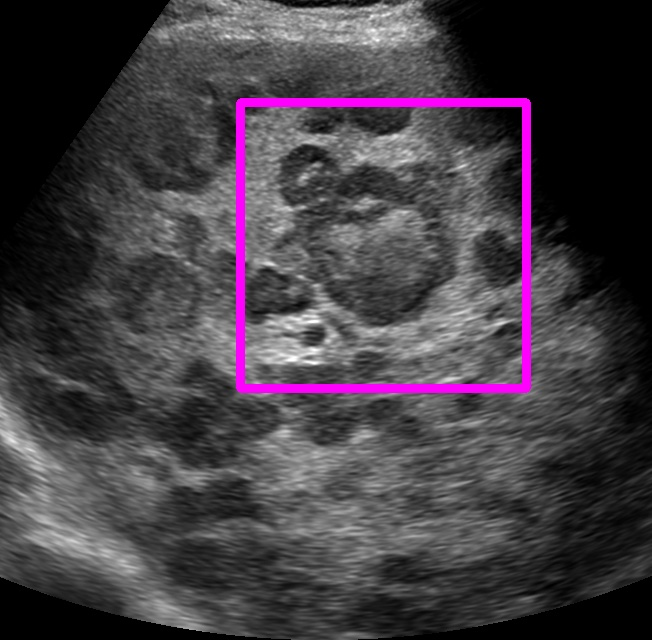
\includegraphics[width=.9\linewidth]{../fig/pseudo_a.png}
            \caption{ラベル不足のある診断画像例}
            \label{fig:ex}
        \end{minipage}
    \end{figure}

    \footnotetext[1]{今回は\Fref{ex}の様なアノテーションが不足しているものを指す}
    \addtocounter{footnote}{1}

    \section{これまでの研究のまとめ}
        \begin{itemize}
            \item データセット
            \begin{itemize}
                \item 国立研究開発法人日本医療研究開発機構(AMED)\footnote{\url{https://www.amed.go.jp/}}が提供している延べ8万枚に及ぶ以下のデータが付随
                \begin{itemize}
                    \item 腹部超音波画像,ROI
                    \item 年齢,性別
                \end{itemize}
                \begin{figure}[h]
                    \centering
                    \subfloat[性別毎の画像枚数]{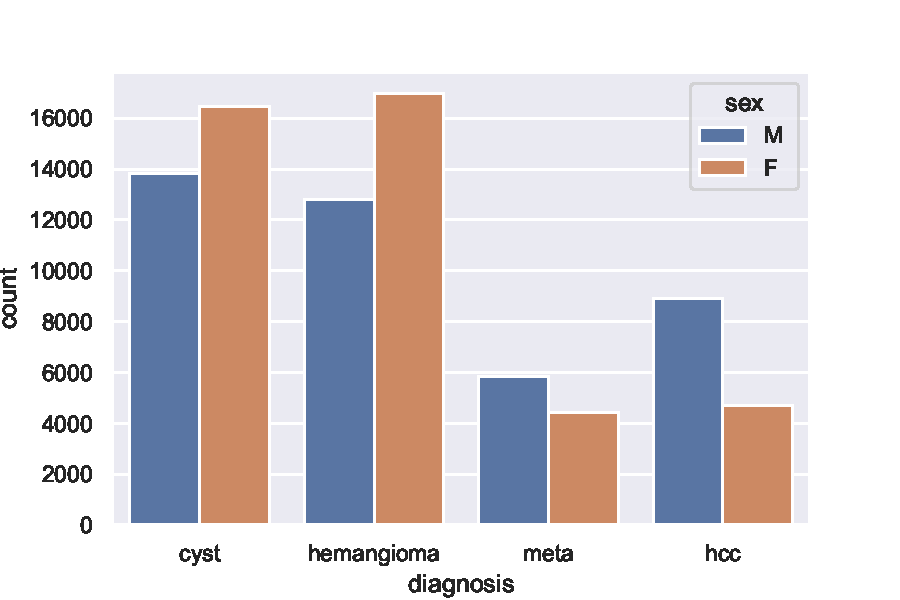
\includegraphics[width=.24\linewidth]{../fig/sex_a.pdf} \label{fig:sex}}
                    \subfloat[診断名毎の年齢分布]{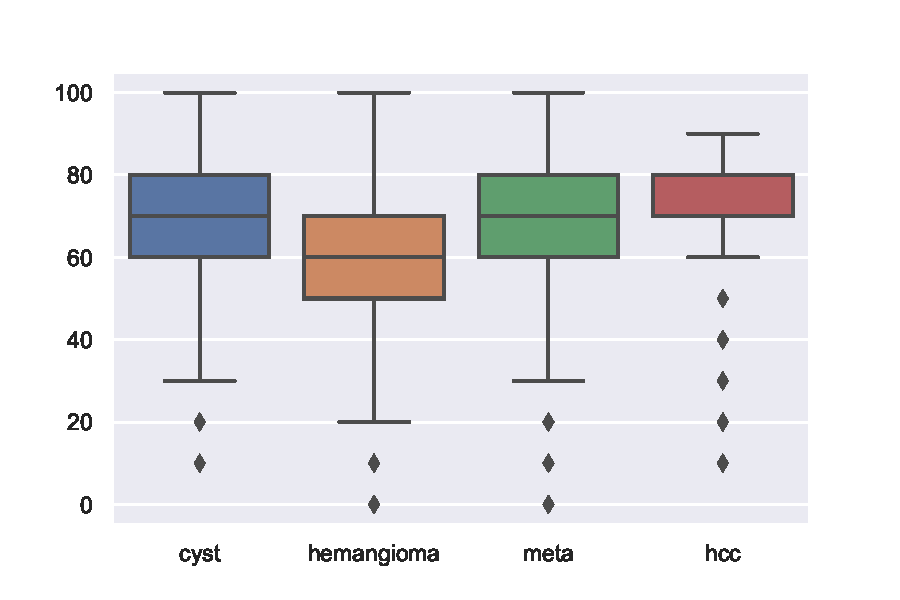
\includegraphics[width=.24\linewidth]{../fig/age_a.pdf} \label{fig:age}}
                    \subfloat[診断名毎の画像サイズの分布]{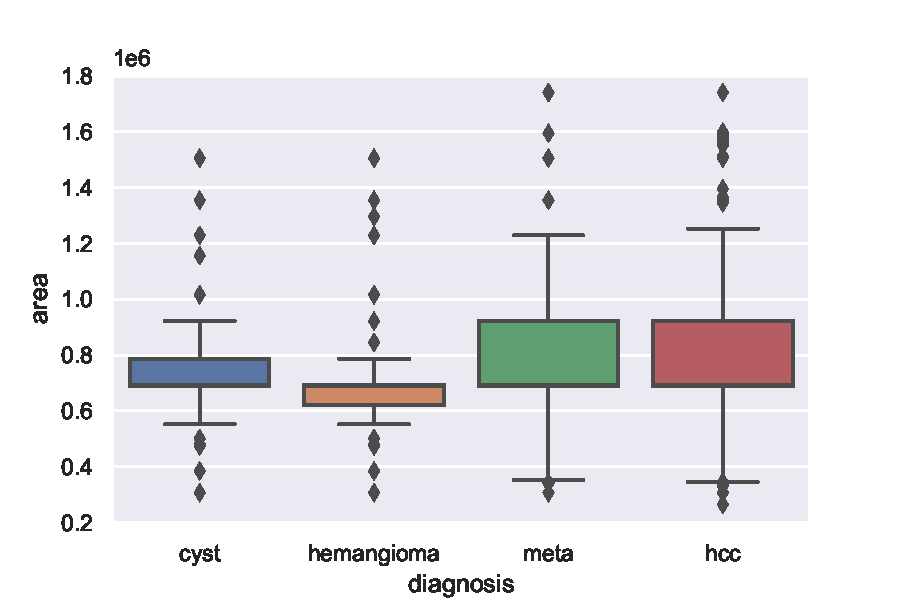
\includegraphics[width=.24\linewidth]{../fig/area_a.pdf} \label{fig:area}}
                    \subfloat[診断名毎のbboxの割合]{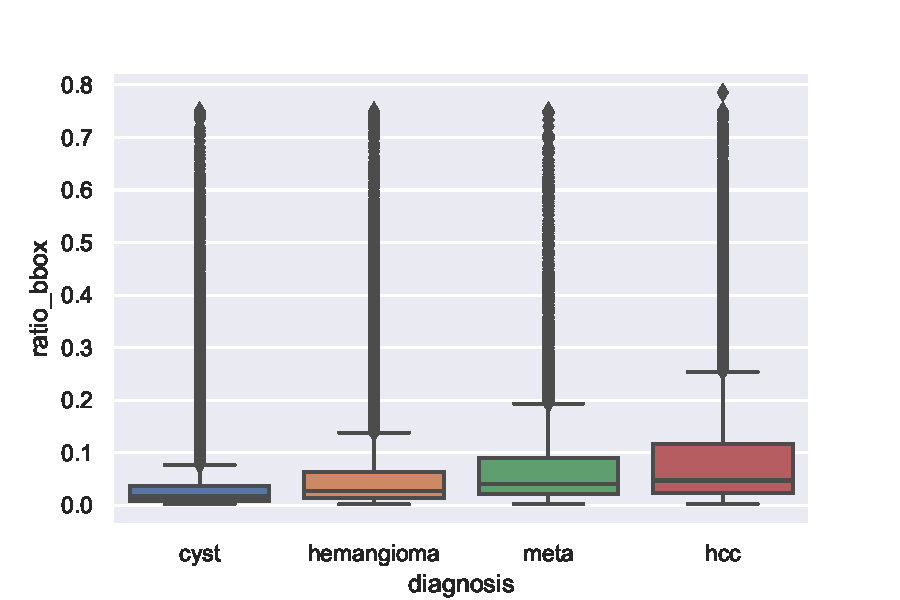
\includegraphics[width=.24\linewidth]{../fig/ratio_bbox_a.pdf} \label{fig:ratio}}
                    \caption{データセットにおけるデータの分布}
                \end{figure}
                \item 性別(\Fref{sex})
                \begin{itemize}
                    \item HCC(肝細胞癌)は男性が罹患しやすい
                    \begin{itemize}
                        \item 昔は男性の方が飲酒・タバコが多く癌に罹りやすかったという時代背景があるかもしれない
                    \end{itemize}
                    \item hemangioma(血管腫)は女性が罹患しやすい
                    \item Meta(転移性肝癌)は他の症状よりも少ない
                \end{itemize}
                \item 年齢(\Fref{age})
                \begin{itemize}
                    \item cyst(単純嚢胞),hemangioma(血管腫)の分布にははあまり特徴がない
                    \item hemangioma(血管腫)は比較的若年層でも罹患する
                    \item Meta(転移性肝癌)における0歳はラベルミスである可能性が高い
                    \item HCC(肝細胞癌)は比較的高齢者が罹患しやすい
                \end{itemize}
                \item 画像サイズ(\Fref{area})
                \begin{itemize}
                    \item hemangioma(血管腫)は比較的画像サイズが統一されている
                    \begin{itemize}
                        \item 腫瘍の大きさが血管に依存するためあまり偏りが生じていない?
                    \end{itemize}
                \end{itemize}
                \item bboxの画像に占める割合(\Fref{ratio})
                \begin{itemize}
                    \item cyst(単純嚢胞)は他の診断と比べてbboxの割合が低い($\frac{1}{2}$程度)である
                    \item HCC(肝細胞癌)は画像に占めるbboxの割合が高い
                \end{itemize}
            \end{itemize}
        \end{itemize}

        \begin{itemize}
            \item 症状毎の特徴を調査
            \begin{figure}[h]
                \centering
                \subfloat[cyst(単純嚢胞)]{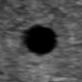
\includegraphics[width=.24\linewidth]{../fig/cyst.png} \label{fig:cyst}}
                \subfloat[hemangioma(血管腫)]{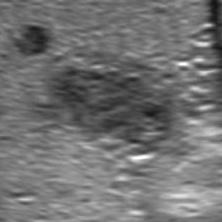
\includegraphics[width=.24\linewidth]{../fig/hemangioma.png} \label{fig:hemangioma}}
                \subfloat[Meta(転移性肝癌)]{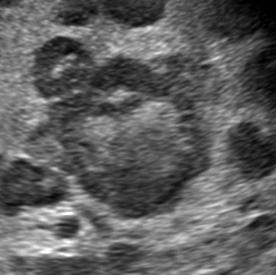
\includegraphics[width=.24\linewidth]{../fig/meta.png} \label{fig:meta}}
                \subfloat[HCC(肝細胞癌)]{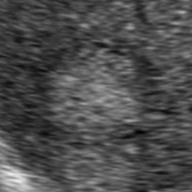
\includegraphics[width=.24\linewidth]{../fig/hcc.png} \label{fig:hcc}}
                \caption{症状毎における腫瘍の超音波画像}
            \end{figure}
            \begin{itemize}
                \item cyst(単純嚢胞) (\Fref{cyst})
                \begin{itemize}
                    \item 液体が貯留されている状態
                    \item 症状がでないことが多いため大きな腫瘍になって発見されることが多い
                    \item 嚢胞の内腔に向けて増殖するため転移することは少ない
                \end{itemize}
                \item hemangioma(血管腫) (\Fref{hemangioma})
                \begin{itemize}
                    \item 肝臓にできる良性腫瘍の中で最も多い
                    \item 女性ホルモンが原因で女性が罹患しやすいと言われているが詳しくは解明されていない
                    \item 血管が無数に絡み合うことによって出来た血管の塊であることから血流が遅いという特徴がある
                    \item 他の臓器に浸潤したり転移することは無いと言われている
                \end{itemize}
                \item Meta(転移性肝癌) (\Fref{meta})
                \begin{itemize}
                    \item 門脈を介して大腸癌などの消化器癌から転移する割合が多い
                    \item 類似したエコーパターンをもつ腫瘤が多発してみられることが多い
                \end{itemize}
                \item HCC(肝細胞癌) (\Fref{hcc})
                \begin{itemize}
                    \item 肝臓にできる悪性腫瘍の中で最も多いと言われている
                    \item 約90%がウイルス感染症が原因
                    \begin{itemize}
                        \item B型肝炎ウイルス(HBV)が約20\%
                        \item C型肝炎ウイルス(HCV)が約70\%
                    \end{itemize}
                \end{itemize}
            \end{itemize}
        \end{itemize}

        \begin{itemize}
            \item データクレンジング
            \begin{enumerate}
                \item $400 \times 400$ 以下の画像の除外
                \item Perceptual Hashを利用した類似画像の除外
                \item 青色や黄色のスケールの除去
            \end{enumerate}

            \item 提供されているデータをCOCODatasetの形式に変換
            \begin{itemize}
                \item train data : test data : val data = 67122 : 8390 : 8391
                \item 見やすいようにインデントしたファイル\footnote{\url{//aka/work/hara.e/AMED/lib/dataset/annotations/train_large.json}など}も作成
            \end{itemize}

\clearpage

            \item 1クラス (腫瘍) での学習結果
                \begin{figure}[h]
                    \centering
                    \subfloat[loss]{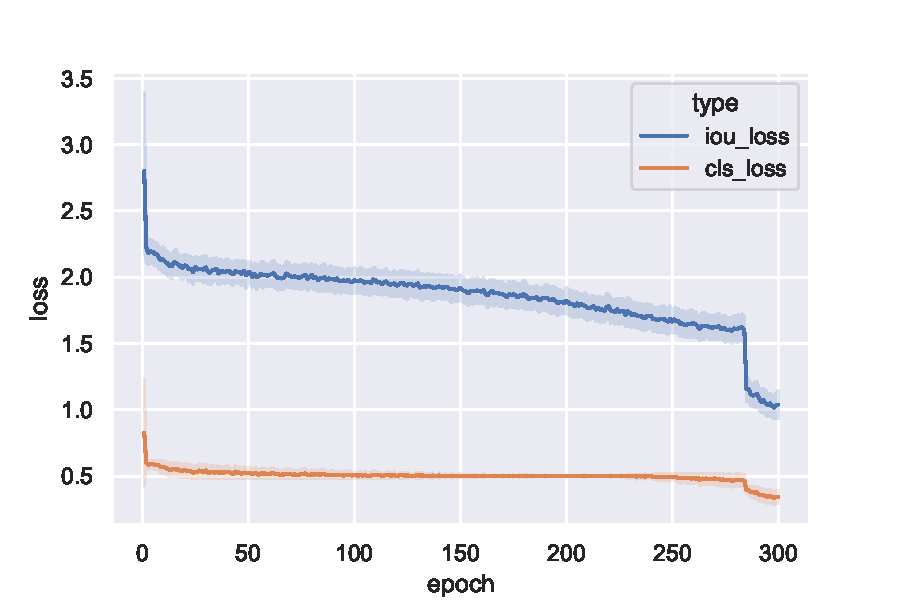
\includegraphics[width=.56\linewidth]{../fig/yoloxs1_loss.pdf} \label{fig:loss}}
                    \subfloat[PR曲線]{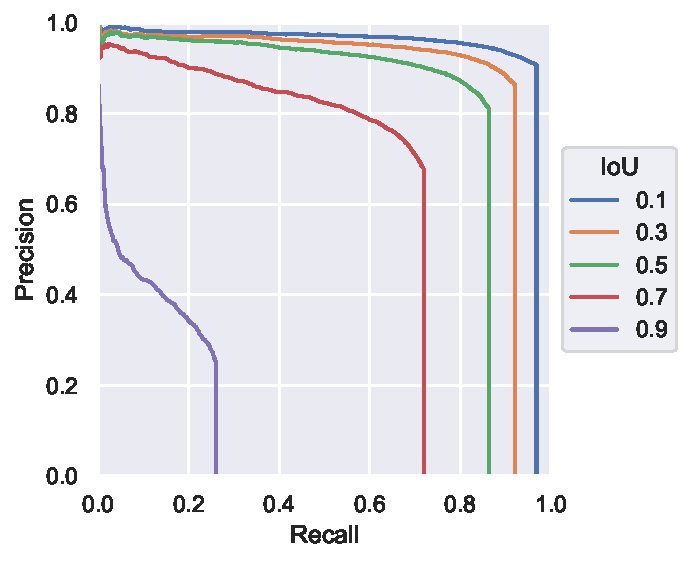
\includegraphics[width=.42\linewidth]{../fig/pr-curve.pdf}
                    \label{fig:pr}}
                    \caption{YOLOX\cite{yolox}で1クラスの検出を行った時のlossとPR曲線}
                \end{figure}

                \begin{table}[h]
                    \centering
                    \caption{1クラスの学習で得られた精度}
                    \label{tab:exp}
                    \begin{tabular}{cccccc|ccc|ccc}
                        & & & & & & & IoU & & & area \footnotemark & \\
                        model & backbone & classes & epoch & size & batch\_size & mAP & AP$_{50}$ & AP$_{75}$ & AP$_S$ & AP$_M$ & AP$_L$ \\ \hline
                        YOLOX\cite{yolox} & DarkNet & 1 & 300 & 512 & 64 & 0.519 & 0.839 & 0.558 & - & 0.639 & 0.631 \\
                    \end{tabular}
                \end{table}

            \item 考察
            \begin{itemize}
                \item \Fref{loss}から
                \begin{itemize}
                    \item IoUのlossがclass分類のlossに比べて大きい
                    \begin{itemize}
                        \item 1クラス分類のためcls\_lossは小さくなる傾向がある
                        \item Noisy Labelの影響?
                    \end{itemize}
                    \item IoUのlossでより大きなDouble Descent\cite{double_descent}が起きている
                    \begin{itemize}
                        \item Noisy Labelが最大の要因
                        \item iou\_lossとcls\_lossはbockboneとしてDarkNetを共有していることからcls\_lossにも影響が出ている?
                    \end{itemize}
                \end{itemize}
                \item \Fref{pr}から
                \begin{itemize}
                    \item RecallがPrecisionに比べて低い
                    \begin{itemize}
                        \item Recallが低いということは腫瘍を検出できていないということ
                        \item 医用でRecallが低いのは問題
                    \end{itemize}
                \end{itemize}
            \end{itemize}
        \end{itemize}
        \footnotetext{Small $< 32^2 <$ Medium $<96^2<$ Large}

\clearpage

    \section{前回のGMからの進捗}
        \begin{itemize}
            \item 4クラス分類での学習結果

            \begin{figure}[h]
                \centering
                \subfloat[AP]{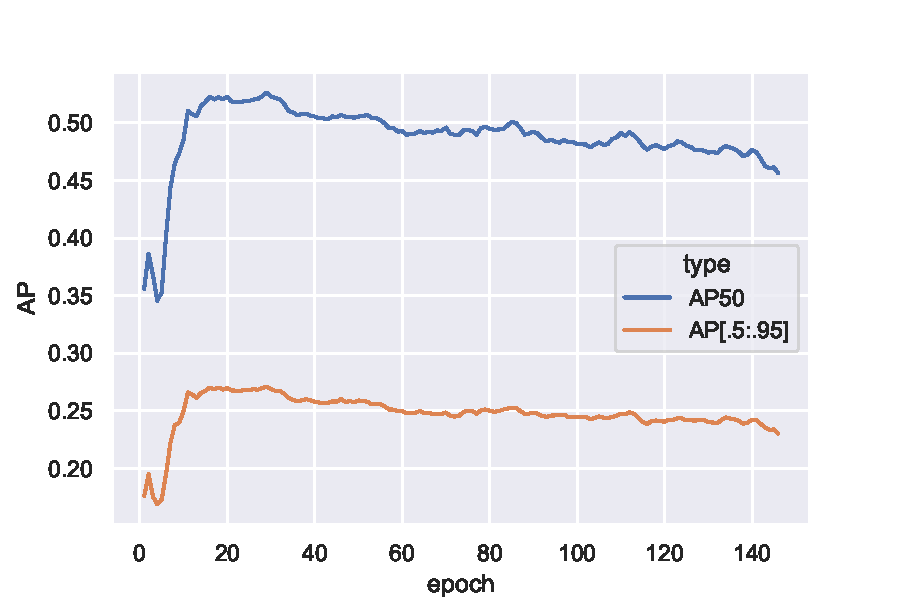
\includegraphics[width=.32\linewidth]{../fig/yoloxs4_AP.pdf} \label{fig:yoloxs4_AP}}
                \subfloat[loss]{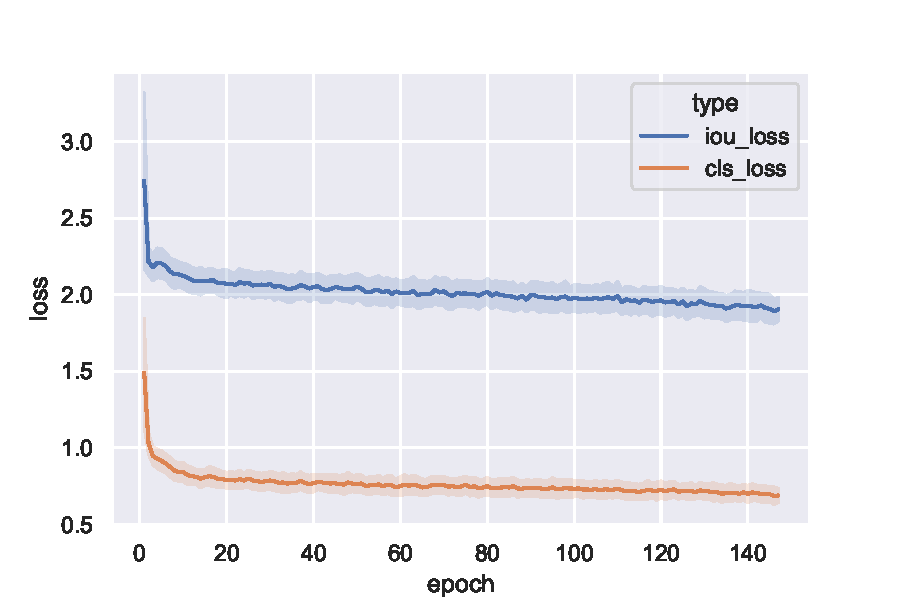
\includegraphics[width=.32\linewidth]{../fig/yoloxs4_loss.pdf}
                \label{fig:yoloxs4_loss}}                
                \subfloat[混同行列]{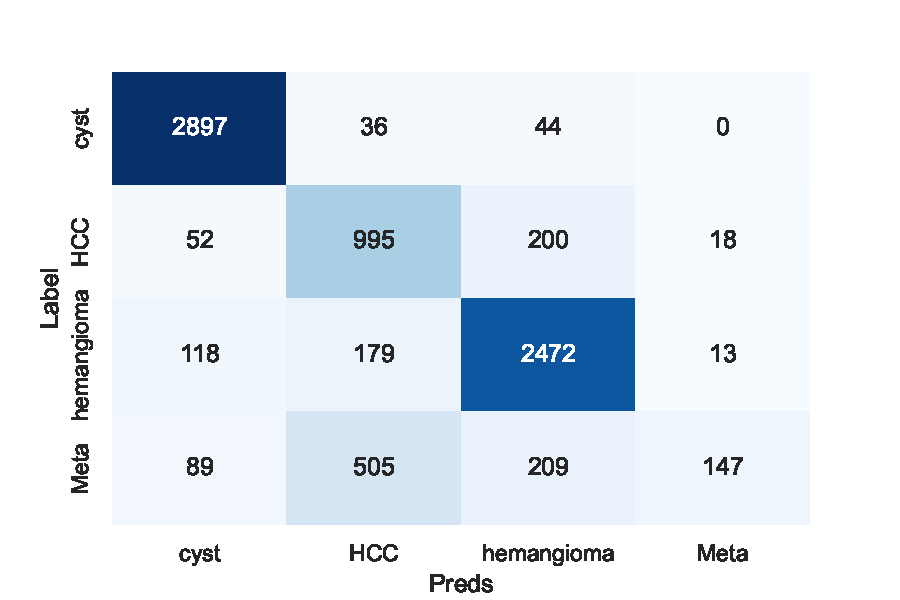
\includegraphics[width=.32\linewidth]{../fig/heatmap.pdf}
                \label{fig:heatmap}}
                \caption{YOLOX\cite{yolox}で4クラス分類を行った時のAPとlossおよび混同行列}
            \end{figure}

            \begin{table}[h]
                \centering
                \caption{4クラス分類を行った時の未検出数}
                \label{tab:undetected}
                \begin{tabular}{c|cccc}
                    Diagnosis & cyst & HCC & hemangioma & Meta \\ \hline
                    未検出数 & 60 & 106 & 180 & 71 \\
                    データ総数 & 3037 & 1371 & 2962 & 1021 \\ \hline
                    未検出割合 & 0.0198 & \textcolor{red}{0.0773} & \textcolor{red}{0.0608} & \textcolor{red}{0.0695}
                \end{tabular}
            \end{table}

            \begin{itemize}
                \item \Fref{yoloxs4_AP}から
                \begin{itemize}
                    \item 30epoch辺りから過学習が起きている
                \end{itemize}
                \item \Fref{yoloxs4_loss}から
                \begin{itemize}
                    \item IoUが精度を下げている大きな要因
                \end{itemize}
                \item \Tref{undetected}から
                \begin{itemize}
                    \item cyst (単純嚢胞) は比較的未検出数が少ない
                \end{itemize}
                \item \Fref{heatmap}と\Tref{undetected}から\Tref{heatmap}の様な値を得ることができる

                \begin{table}[h]
                    \centering
                    \caption{評価指標毎の値}
                    \label{tab:heatmap}
                    \begin{tabular}{c|cccc}
                        Diagnosis & accuracy & precision & recall & f1-score \\ \hline
                        cyst & 0.8789 & 0.9179 & 0.9539 & 0.9356 \\
                        HCC & 0.4758 & \textcolor{red}{0.5801} & 0.7257 & 0.6448 \\
                        hemangioma & 0.7238 & 0.8451 & 0.8346 & 0.8398 \\
                        Meta & \textcolor{red}{0.1397} & 0.8258 & \textcolor{red}{0.1440} & \textcolor{red}{0.2452} \\
                    \end{tabular}
                \end{table}

                \item \Tref{heatmap}から
                \begin{itemize}
                    \item 精度が要求される診断名の精度が低い
                    \begin{itemize}
                        \item 実用上最も問題がある診断名はMeta (転移性肝癌)
                        \item 予測が最も信用出来ない診断名はHCC (肝細胞癌)
                    \end{itemize}
                \end{itemize}
                \item まとめ
                \begin{itemize}
                    \item cyst (単純嚢胞)
                    \begin{itemize}
                        \item ほぼ問題ない
                    \end{itemize}
                    \item hemangioma (血管腫)
                    \begin{itemize}
                        \item cyst (単純嚢胞) やHCC (肝細胞癌) と誤分類してしまうことが多い
                        \item 未検出の多さが目立つ
                    \end{itemize}
                    \item HCC (肝細胞癌)
                    \begin{itemize}
                        \item hemangioma (血管腫) と誤分類してしまうことが多い
                        \item \textcolor{red}{未検出が多い}
                    \end{itemize}
                    \item Meta (転移性肝癌)
                    \begin{itemize}
                        \item HCC (肝細胞癌) やhemangioma (血管腫) と誤分類してしまうことが多い
                        \item \textcolor{red}{正確な予測ができていない} (予測がバラバラ) ことが多い
                    \end{itemize}
                \end{itemize}
            \end{itemize}

\clearpage

            \item 1クラス分類と4クラス分類の比較

            \begin{figure}[h]
                \centering
                \subfloat[APの比較]{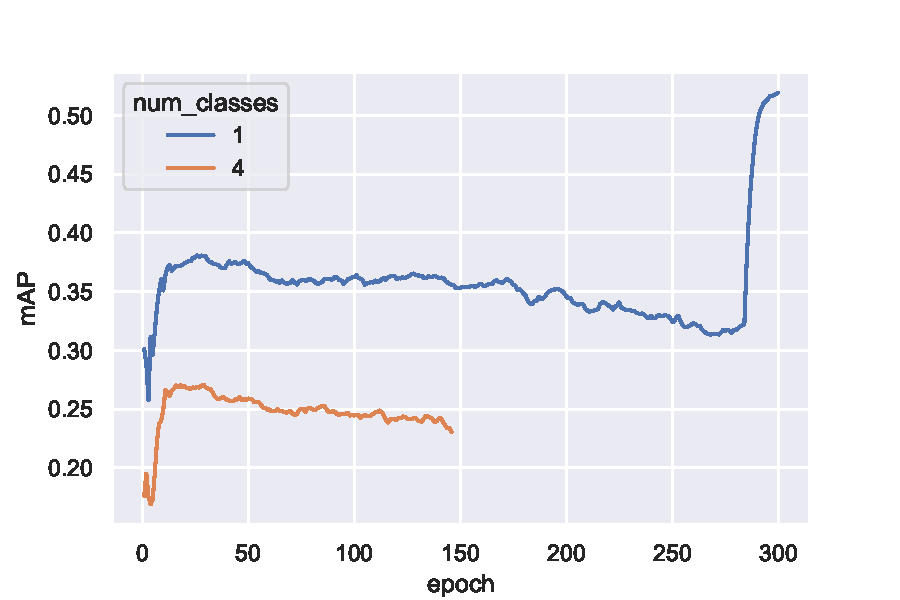
\includegraphics[width=.32\linewidth]{../fig/compare_AP.pdf} \label{fig:compare_AP}}
                \subfloat[iou\_lossの比較]{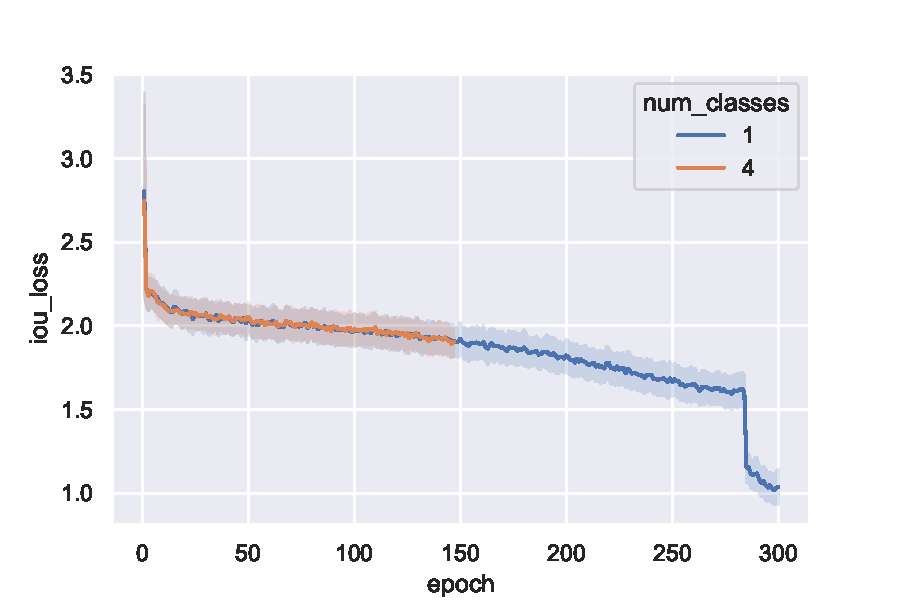
\includegraphics[width=.32\linewidth]{../fig/compare_iou_loss.pdf} \label{fig:compare_iou_loss}}\subfloat[cls\_lossの比較]{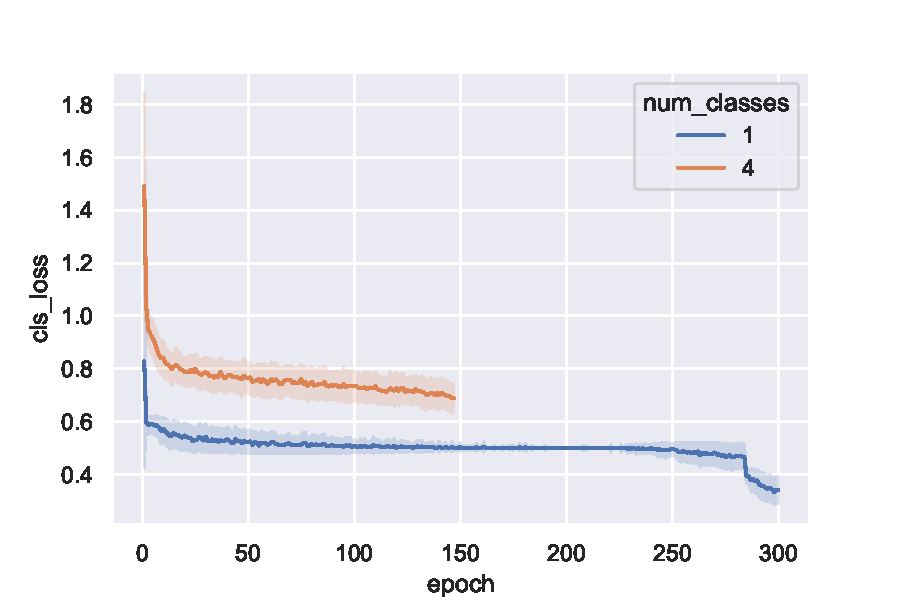
\includegraphics[width=.32\linewidth]{../fig/compare_cls_loss.pdf} \label{fig:compare_cls_loss}}
                \label{fig:compare}
                \caption{1クラス分類と4クラス分類の比較}
            \end{figure}

            \begin{itemize}
                \item \Fref{compare_AP}から
                \begin{itemize}
                    \item 4クラス分類の方がAPが低い
                    \item クラス数を増やしているから当たり前
                \end{itemize}
                \item \Fref{compare_iou_loss}から
                \begin{itemize}
                    \item 1クラスと4クラスは同じくらいの学習速度
                    \item 1クラスと4クラスではiou\_lossの差異が小さい
                    \item クラス数を増やしてもIoUの精度はあまり変化が無い
                \end{itemize}
                \item \Fref{compare_cls_loss}から
                \begin{itemize}
                    \item 1クラスと4クラスではcls\_lossの差異が大きい
                    \item クラス数を増やしているから当たり前
                \end{itemize}

                \begin{table}[h]
                    \centering
                    \caption{1クラスと4クラスの学習で得られた精度}
                    \label{tab:compare}
                    \begin{tabular}{cccccc|ccc|ccc}
                        & & & & & & & IoU & & & area & \\
                        model & backbone & classes & epoch & size & batch\_size & mAP & AP$_{50}$ & AP$_{75}$ & AP$_S$ & AP$_M$ & AP$_L$ \\ \hline
                        \multirow{2}{*}{YOLOX\cite{yolox}} & \multirow{2}{*}{DarkNet} & 1 & \multirow{2}{*}{300} & \multirow{2}{*}{512} & \multirow{2}{*}{64} & 0.519 & 0.839 & 0.558 & - & 0.639 & 0.631 \\
                        &  & 4 &  &  &  & 0.279 & 0.526 & 0.248 & - & 0.221 & 0.288 \\
                    \end{tabular}
                \end{table}

                \item \Tref{compare}から
                \begin{itemize}
                    \item APが半分程度になっている
                    \item IoUが0.5の時はAPが比較的高い
                    \item 4クラス分類では腫瘍が大きいものは分類しやすい傾向がある?
                \end{itemize}
            \end{itemize}

\clearpage

            \item これから用いるモデルについて考えた
            \begin{figure}[h]
                \centering
                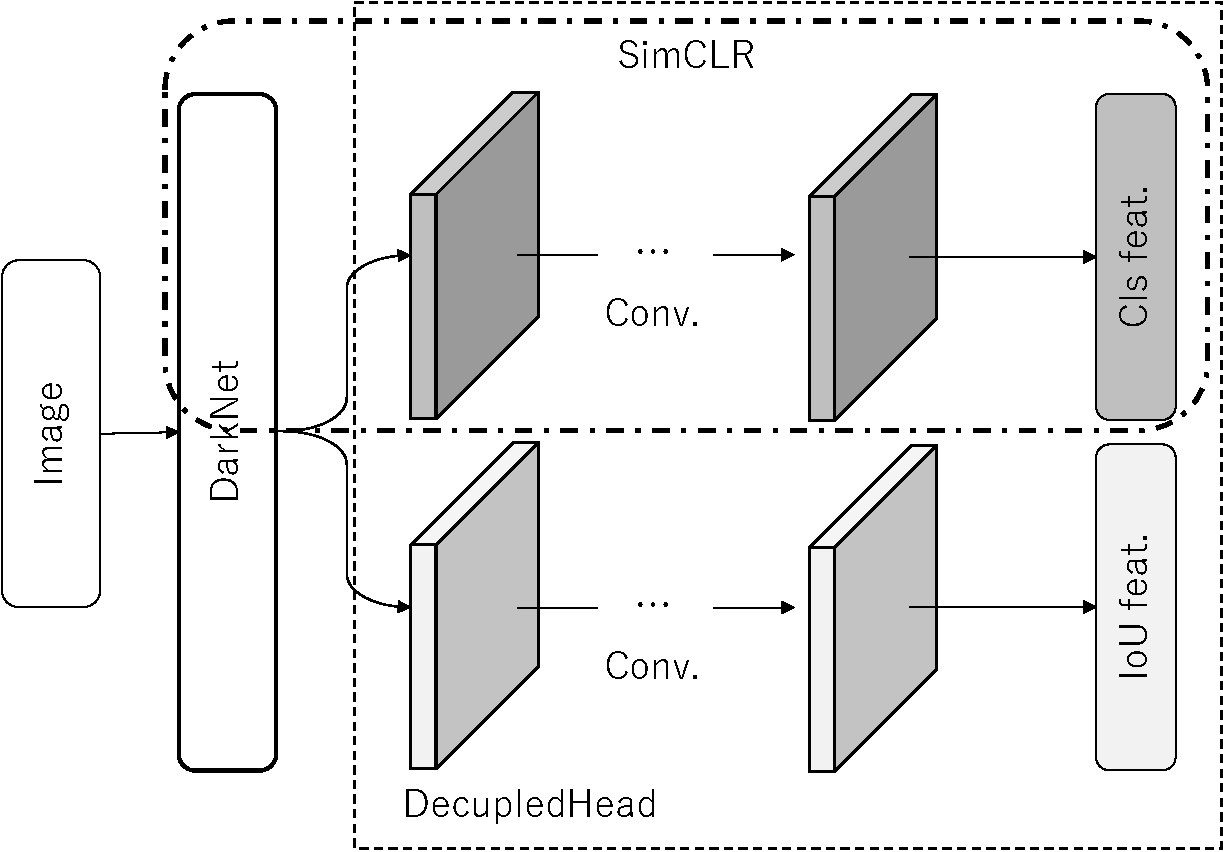
\includegraphics[width=.73\linewidth]{../fig/model.pdf}
                \caption{YOLOX\cite{yolox}とSimCLR\cite{simclr}の複合モデル}
                \label{fig:model}
            \end{figure}
            \begin{itemize}
                \item クラス分類の部分のmodelをSimCLR\cite{simclr}で事前学習
                \item 一部 (クラスの特徴量を抽出する層) だけfreezeする
            \end{itemize}
            \item SimCLR\cite{simclr}を使ってみた
            \begin{itemize}
                \item ハイパーパラメーター
                \begin{itemize}
                    \item backbone: ResNet18
                    \item batch\_size: 256
                    \item epoch数: 200
                    \item size: (96, 96)
                \end{itemize}
            \end{itemize}

            \begin{figure}[h]
                \centering
                \subfloat[accuracy]{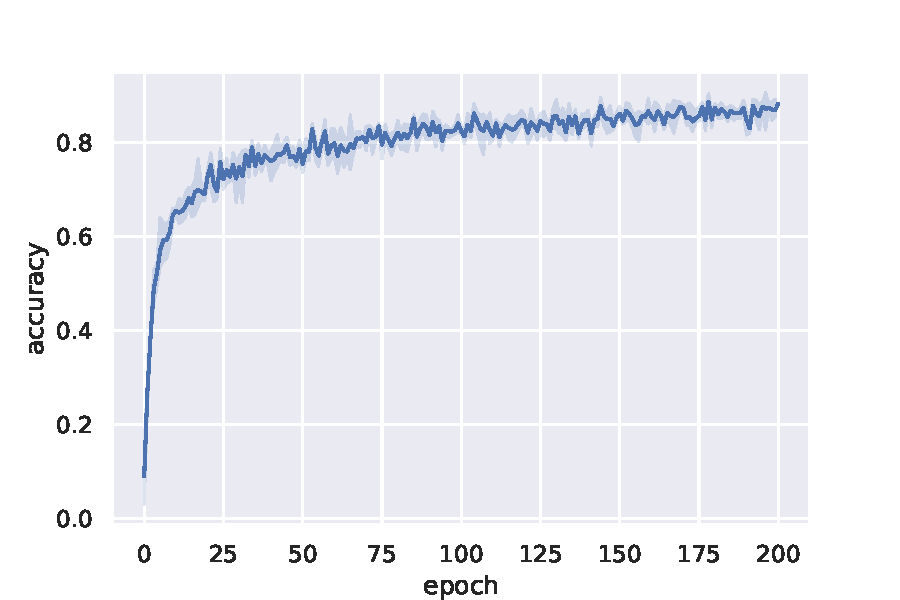
\includegraphics[width=.49\linewidth]{../fig/simclr_acc_res.pdf} \label{fig:simclr_acc}}
                \subfloat[loss]{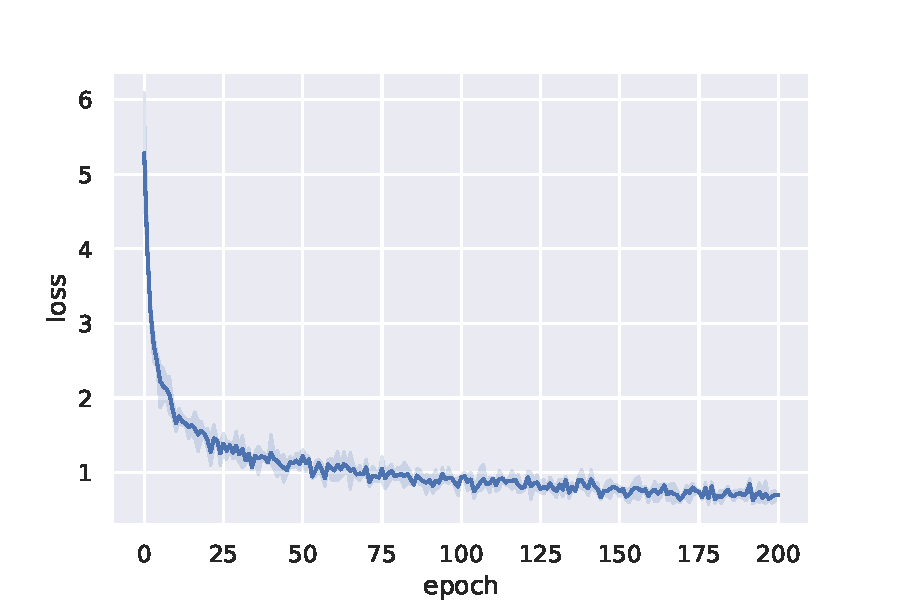
\includegraphics[width=.49\linewidth]{../fig/simclr_loss_res.pdf}
                \label{fig:simclr_loss}}
                \caption{SimCLR\cite{simclr}で対照学習を行なった結果 (trainデータ)}
            \end{figure}

            % \begin{table}[h]
            %     \centering
            %     \caption{対照学習で得られた精度}
            %     \label{tab:metric}
            %     \begin{tabular}{ccc|ccc}
            %         model & backbone & classes & accuracy & recall & precision \\ \hline
            %         SimCLR\cite{simclr} & ResNet18 & 4 & 0.519 & 0.839 & 0.001 \\
            %     \end{tabular}
            % \end{table}

        \end{itemize}

\clearpage

    \section{今後の課題\&スケジュール}
        \begin{itemize}
            \item 5/31までに
            \begin{itemize}
                \item 対照学習の結果を (遅くとも6/14までに) 出すことを目標にする
                \item 結果と言っても (できれば同じbackboneを使って) testデータでPrecisionやRecallを出すところまで
            \end{itemize}
        \end{itemize}

    \begin{thebibliography}{9}
        \bibitem{double_descent} Anonymous authors. \href{https://openreview.net/attachment?id=B1g5sA4twr&name=original_pdf}{DEEP DOUBLE DESCENT: WHERE BIGGER MODELS AND MORE DATA HURT} ICLR 2020, 2020.
        \bibitem{yolox} Zheng Ge, Songtao Liu, Feng Wang, Zeming Li, and Jian Sun. \href{https://arxiv.org/pdf/2107.08430.pdf}{YOLOX: Exceeding YOLO Series in 2021}, 2021.
        \bibitem{simclr} Ting Chen, Simon Kornblith, Mohammad Norouzi, Geoffrey Hinton. \href{https://arxiv.org/pdf/2002.05709.pdf}{A Simple Framework for Contrastive Learning of Visual Representations}, 2020.
    \end{thebibliography}
\end{document}